%\section{Introduction}
\section{Position du problème}
\label{sec:introfacto}

% \ANNOT{...\cite{Pom96} \cite{BahiC06} \cite{Fat13}... citations liées à la factorisation ...
% }


On cherche un système dynamique discret qui, étant donné un entier non-premier, trouve un de ses diviseurs non-triviaux. On se base sur la multiplication binaire. En effet, on observe qu'une matrice à coefficients dans $\{0,1\}$ peut s'interpréter comme une multiplication binaire si ses lignes non-nulles sont égales entre elles, comme illustré dans la Figure~\ref{fig:ExShift}. Les colonnes non-nulles sont alors aussi égales entre elles, et les deux facteurs de la multiplication sont alors lisibles, en base~$2$, sur les lignes non-nulles pour l'un, et de bas en haut sur les colonnes non-nulles pour l'autre. Si on pose leur multiplication, toujours en base~$2$, on retrouve en effet la matrice de départ décalée d'un cran par ligne vers la gauche (cf. Figure~\ref{fig:ExShift}).




\begin{figure}[h]
\centering
\begin{minipage}[]{0.25\linewidth}
$M=$
\begin{tabular}{cccc}
1&0&1&1\\
0&0&0&0\\
1&0&1&1\\
1&0&1&1\\
\end{tabular}

\end{minipage}
\quad
\begin{minipage}[]{0.4\linewidth}


\begin{tabular}{lllllllll|c}
&&&&&1&0&1&1&$\times$\\
\hline
&&&&&1&0&1&1&1\\
+&&&&0&0&0&0&.&0 \\
+&&&1&0&1&1&.&.&1\\
+&&1&0&1&1&.&.&.&1\\
\hline
$\sigma(M)=$&1&0&0&0&1&1&1&1&143\\
\end{tabular}
\end{minipage}
\caption{La matrice M s'interprète comme la multiplication de $11$ ($1011$ horizontalement) par $13$ ($1101$ verticalement, de haut en bas), et le produit est $\sigma(M)=143$.}
\label{fig:ExShift}
\end{figure}

%\ANNOT{Fusionner la figure 10 avec la figure 9 en complétant la légende aussi.}

\begin{df*}
Étant donné une matrice~$M$ à coefficients dans $\{0,1\}$, on appelle \emph{somme} de~$M$ et on note $\sigma (M)$ l'entier obtenu en sommant ses lignes décalées (cf. Figure~\ref{fig:ExShift}). Si~$M$ représente une multiplication, $\sigma(M)$ est par construction le produit. 
\end{df*}


% \begin{figure}[]
% \centering
% \begin{minipage}[]{0.3\linewidth}
% $M=$
% \begin{tabular}{cccc}
% 1&1&0&1\\
% 0&0&1&1\\
% 1&0&0&1\\
% \end{tabular}
% \end{minipage}
% \quad
% \begin{minipage}[]{0.45\linewidth}
% $\sigma(M)=$
% \begin{tabular}{llllllll}
% &&&&1&1&0&1\\
% +&&&0&0&1&1&.\\
% +&&1&0&0&1&.&.\\
% \hline
% &&1&1&0&1&1&1\\
% \end{tabular}
% $=55$
% \end{minipage}
% \caption{Exemple de calcul de $\sigma$.}
% \label{fig:ExSigma}
% \end{figure}

L'idée est donc de partir d'une matrice à coefficients dans $\{0,1\}$ dont la somme vaut le nombre qu'on cherche à factoriser, et de lui appliquer des transformations qui préservent la somme comme invariant jusqu'à atteindre une matrice qui représente une multiplication. Ainsi, notre système n'a pas à vérifier que le produit de cette multiplication est l'entier à factoriser, ce qui simplifie considérablement sa conception.

\section{Un algorithme}

Soit~$n$ le nombre de chiffres en base~$2$ du nombre composé~$N$ dont on cherche un diviseur non-trivial. On se donne une matrice~$M$ de taille $ n-1 \times \lceil \frac{n}{2}\rceil$ de somme~$N$. Pour tous~$a$ et~$b$ différents de~$1$ et~$N$, et tels que $N = ab$,~$a$ ou~$b$ est de taille inférieure à $\lceil\frac{n}{2}\rceil$ et l'autre est de taille inférieure à $n-1$, on peut donc représenter leur multiplication à l'aide d'une matrice de la taille de~$M$. On l'initialise en recopiant les $n-1$ bits de poids faible de~$N$ sur la première ligne, et avec un~$1$ en position $(2,1)$ et des zéros partout ailleurs (cf. Figure \ref{fig:init}). On vérifie aisément que $\sigma(M)=N$. 


\begin{figure}[h]
\centering

$21 \Rightarrow \overline{10101}^2 \Rightarrow$
\begin{tabular}{cccc}
0&1&0&1\\
1&0&0&0\\
0&0&0&0\\
\end{tabular}
$\Rightarrow$
\begin{tabular}{ccccccc}
&&&0&1&0&1\\
+&&1&0&0&0&.\\
+&0&0&0&0&.&.\\
\hline
&0&1&0&1&0&1\\
\end{tabular}

\caption{Exemple de construction de la matrice~$M$ de départ pour factoriser $N=21$.}
\label{fig:init}
\end{figure}

Formellement, on pose $\La=\cg 1, n-1 \cd \times \cg 1, \lceil\frac{n}{2}\rceil\cd$ l'ensemble des cases de la matrice, et $\E=\{0,1\}^\La$ l'ensemble des configurations. Pour tout $x \in \E$, $(i,j)\in\La$, on note $x_{i,j}$ le coefficient $(i,j)$ de la matrice~$x$. 
On se donne également un ensemble $\Gamma \subset \E^{\E\times\La}$ de transformations locales qui préservent l'invariant de somme. Elles sont représentées sur la Figure~\ref{fig:rules}, et s'appliquent aux coefficients indiqués en gras sous certaines conditions. Les règles \textbf{R5} et \textbf{R6} ne sont en fait pas nécessaires pour l'accessibilité des solutions : on les introduit par symétrie, pour ne pas privilégier de direction de déplacements des~$1$. 

%On se donne donc un ensemble $\Gamma$ de six transformations locales qui conservent $\sigma$. Elles sont représentées sur la figure~$3$. Plus 

\begin{figure}[hbt]
\centering

\resizebox{\textwidth}{!}{
\begin{minipage}{0.4\textwidth}
\[
\begin{pmatrix}
.&.&\textbf 1&.\\
.&.&.&0\\
.&.&.&.\\
\end{pmatrix}
\mathrel{\mathop{\longrightleftarrows}^{\mathrm{R1}}_{\mathrm{R2}}}
\begin{pmatrix}
.&.&\textbf 0&.\\
.&.&.&1\\
.&.&.&.\\
\end{pmatrix}
\]

\[
\begin{pmatrix}
.&.&0&.\\
.&\textbf 1&0&.\\
.&.&.&.\\
\end{pmatrix}
\mathrel{\mathop{\longrightleftarrows}^{\mathrm{R3}}_{\mathrm{R4}}}
\begin{pmatrix}
.&.&1&.\\
.&\textbf 0&1&.\\
.&.&.&.\\
\end{pmatrix}
\]

\[
\begin{pmatrix}
.&\textbf 1&0&.\\
.&.&.&0\\
.&.&.&.\\
\end{pmatrix}
\mathrel{\mathop{\longrightleftarrows}^{\mathrm{R5}}_{\mathrm{R6}}}
\begin{pmatrix}
.&\textbf 0&1&.\\
.&.&.&1\\
.&.&.&.\\
\end{pmatrix}
\]%

% \[
% \begin{tabular}{cc}
% \textbf 1&\\
% &0\\
% &\\
% \end{tabular}
% \mathrel{\mathop{\longrightleftarrows}^{\mathrm{R1}}_{\mathrm{R2}}}
% \begin{tabular}{cc}
% \textbf 0&\\
% &1\\
% &
% \end{tabular}
% \]

% \[
% \begin{tabular}{cc}
% \textbf 1&\\
% &0\\
% &
% \end{tabular}
% \mathrel{\mathop{\longrightleftarrows}^{\mathrm{R1}}_{\mathrm{R2}}}
% \begin{tabular}{cc}
% \textbf 0&\\
% &1\\
% &
% \end{tabular}
% \]

% \[
% \begin{tabular}{cc}
% \textbf 1&\\
% &0\\
% &
% \end{tabular}
% \mathrel{\mathop{\longrightleftarrows}^{\mathrm{R1}}_{\mathrm{R2}}}
% \begin{tabular}{cc}
% \textbf 0&\\
% &1\\
% &
% \end{tabular}
% \]


\end{minipage}
\qquad
\begin{minipage}{0.6\textwidth}
\[
\begin{tabular}{lllllll}
&&&.&.&\textbf 1&. \\
+&&.&.&.&0&\\
+&.&.&.&.&&\\
\hline
\end{tabular}
\mathrel{\mathop{\longrightleftarrows}^{\mathrm{R1}}_{\mathrm{R2}}}
\begin{tabular}{lllllll}
&&&.&.&\textbf 0&. \\
+&&.&.&.&1&\\
+&.&.&.&.&&\\
\hline
\end{tabular}
\]

\[
\begin{tabular}{lllllll}
&&&.&.&0&. \\
+&&.&.&\textbf 1&0&\\
+&.&.&.&.&&\\
\hline
\end{tabular}
\mathrel{\mathop{\longrightleftarrows}^{\mathrm{R3}}_{\mathrm{R4}}}
\begin{tabular}{lllllll}
&&&.&.&1&. \\
+&&.&.&\textbf 0&1&\\
+&.&.&.&.&&\\
\hline
\end{tabular}
\]

\[
\begin{tabular}{lllllll}
&&&.&\textbf 1&0&. \\
+&&.&.&.&0&\\
+&.&.&.&.&&\\
\hline
\end{tabular}
\mathrel{\mathop{\longrightleftarrows}^{\mathrm{R5}}_{\mathrm{R6}}}
\begin{tabular}{lllllll}
&&&.&\textbf 0&1&. \\
+&&.&.&.&1&\\
+&.&.&.&.&&\\
\hline
\end{tabular}
\]
%\caption{Illustration.}
\end{minipage}}

\caption{Transformations locales préservant l'invariant de somme sur un exemple
  de 3 lignes et 4 colonnes.}

\label{fig:rules}

\end{figure}


%À chaque pas de temps, on choisit au hasard une case et une transformation de $\Gamma$, et on décide si on applique ou non la transformation.

Une  formulation  équivalente  de  l'égalité  des lignes  non-nulles  est  qu'un
coefficient situé sur la même ligne qu'un  1 et sur la même colonne qu'un 1 vaut
nécessairement 1 dans une matrice  qui représente une multiplication. On va donc
appliquer  aléatoirement des  règles  conservant $\sigma$,  en privilégiant  les
mouvements qui retirent les zéros de telles cases. Dans la suite, on dira qu'une
case est \emph{sûre}  s'il n'y a pas de~$1$  sur la même ligne ou s'il  n'y en a
pas sur la même  colonne, et \emph{dangereuse} s'il y a à  la fois un~$1$ sur la
même ligne et un sur la même colonne.

\begin{floatingfigure}[r]{0.5\textwidth}
\centering
\begin{tabular}{cccccccc}
0&1&0&0&1&1&0&\fbox 0\\ 
0&\fbox 0&0&0&1&1&0&1\\
0&\fbox 0&0&0&1&1&0&1\\
0&0&0&0&0&0&0&0\\
0&\fbox 0&0&0&1&1&0&1\\
\end{tabular}
\caption{Exemple de situation bloquée si on interdit les mouvements ne déplaçant pas les zéros menacés (encadrés) : aucune des règles de la Figure~\ref{fig:rules} ne s'applique à eux.}
\label{fig:stuck}
\end{floatingfigure}
Pour diriger  les zéros vers  les cases sûres,  on voudrait n'effectuer  que des
mouvements qui sortent un zéro d'une case dangereuse, mais cette restriction est
trop forte : il existe  alors des situations bloquées, la Figure~\ref{fig:stuck}
en  donne un  exemple.  Il est  donc  nécessaire d'autoriser  au moins  certains
mouvements  qui ne  sont pas  directement utiles  en ce  sens. Par  ailleurs, on
pourrait  vouloir   restreindre  les  mouvements   des  zéros  vers   des  cases
dangereuses, de la même façon que pour le problème des~$n$ reines. Cependant, il
se  forme alors  des blocs  stables de~$1$  : les  zéros qui  viennent remplacer
un~$1$  au bord  du bloc  en  sont rapidement  éjectés (les  seules cases  sûres
proches sont à l'extérieur du bloc).
On prend donc le  parti de ne pas restreindre les mouvements  des zéros vers des
cases dangereuses, et on se donne une probabilité d'agitation~$p$ : un mouvement
valide mais qui ne sort pas un  zéro d'une case dangereuse est effectué avec une
probabilité~$p$,  alors qu'un  mouvement  valide  qui sort  un  zéro d'une  case
dangereuse est  toujours effectué. Dans tous  les cas, on ne  s'intéresse pas au
caractère sûr ou dangereux de la case de destination.




À chaque pas de temps, on choisit donc une case de $\La$ et une règle de $\Gamma$ au hasard, et on applique éventuellement la règle à la case. À titre d'exemple, si on choisit, dans une configuration~$x$, la case $(i,j)$ et la règle \textbf{R1}, la nouvelle configuration est \[
\textbf{R1}(x,(i,j))=
\begin{cases}
  \hfill x' \hfill & \text{ si}  \begin{cases}\text{ $x_{i,j}=1$ et $x_{i+1,j+1}=0$ }\\
    \text{ et}  \left\{
        \begin{tabular}{@{}c@{}l}
          &\text{ $(i+1,j+1)$ est une case dangereuse}\\
          \text {ou}&\\
          &\text{ $\mathcal{B}(p)=1$}\\
        \end{tabular}
      \right.
  \end{cases}
  \\
  \hfill x \hfill & \text{ sinon}
\end{cases}
\]

avec $x'$ la configuration obtenue à partir de~$x$ en échangeant les valeurs de $x_{i,j}$ et $x_{i+1,j+1}$, et $\mathcal{B}(p)$ une variable aléatoire valant~$1$ avec une probabilité~$p$ et~$0$ avec une probabilité $1-p$.

On applique une règle si au moins un des zéros concernés est sur une case dangereuse : ainsi \[
\textbf{R3}(x,(i,j))=
\begin{cases}
  \hfill x'' \hfill & \text {si} \begin{cases}\text{ $x_{i,j}=1$ et $x_{i-1,j}=x_{i,j+1}=0$} \\
    \text{ et} \left\{
        \begin{tabular}{@{}c@{}l}
          &\text{ $(i-1,j)$ est une case dangereuse}\\
          \text {ou}& \text{ $(i,j+1)$ l'est}\\
          \text {ou}& \text{ $\mathcal{B}(p)=1$}\\
        \end{tabular}
      \right.
    \end{cases}
  \\
  \hfill x \hfill & \text {sinon}
\end{cases}
\]

avec $x''$ la configuration obtenue à partir de~$x$ en changeant les valeurs de $x_{i,j}$, $x_{i-1,j}$ et $x_{i,j+1}$.


Du fait de l'existence de mouvements spontanés, il n'y a pas de point fixe à proprement parler : on est contraint de vérifier après chaque mouvement si la matrice représente une multiplication valide, et d'arrêter les mises à jour le cas échéant. 

\section{Atteignabilité de la solution}

On cherche ici à montrer que la solution est accessible à partir de toute configuration initiale valide en appliquant uniquement les règles de $\Gamma$. On va en fait montrer un résultat un peu plus général : en appliquant les règles de $\Gamma$, il est possible de passer d'une matrice quelconque à n'importe quelle autre matrice de même somme. On suppose fixée la taille des matrices considérées, mais on ne la suppose pas nécessairement égale à celle qu'on utilise dans l'algorithme : cette généralisation permet d'adapter la preuve à des améliorations de l'algorithme.

\begin{df*}
Pour toutes matrices~$A$ et~$B$, on a $A\sim B$ si et seulement si on peut passer de~$A$ à~$B$ en appliquant des transformations de $\Gamma$.
\end{df*}

Remarquons que $\sim$ est une relation d'équivalence (la symétrie vient du fait que toutes les règles de $\Gamma$ ont un inverse, donc tous les mouvements sont réversibles).



\begin{floatingfigure}[r]{.5\textwidth}
%\begin{figure}[hbt]
\centering
%\begin{tikzpicture}
%\
%\begin{matrix}
%\tikzmark{a} & \tikzmark{b} & \tikzmark{c} & \\
%\phantom{0}\tikzmark{a21}& & \phantom{0}\tikzmark{a23}& b_0 \\
%\phantom{0}\tikzmark{a31}& \phantom{0}\tikzmark{a32} &  \phantom{0}\tikzmark{a33} & b_1 \\
%&b_4&b_3&b_2\\
%\end{matrix}
%\]
%\end{tikzpicture}

\scalebox{0.3}{\subimport{.}{figdiag.pdf_t}}

\caption{Signification des coefficients $b_i$.}
\label{fig:diags}
%\end{figure}
\end{floatingfigure}
Pour toute  matrice~$M$, on numérote  ses diagonales descendantes  en commençant
à~$0$ par celle réduite au coin supérieur droit (cf Fig.~\ref{fig:diags}), et on
note $b_i$ le nombre de coefficients  égaux à~$1$ sur la diagonale~$i$, de sorte
que \linebreak  \mbox{$\sigma (M) = \sum\limits_ib_i2^i$}. On  constate que deux
matrices  ayant  les mêmes  coefficients  $b_i$  pour  \linebreak tout~$i$  sont
équivalentes  pour  $\sim$ (en  fait,  on  peut passer  de  l'une  à l'autre  en
utilisant uniquement les règles \textbf{R1} et \textbf{R2}). On note de plus~$r$
le nombre de diagonales descendantes de  la matrice (si la matrice est de taille
$n\times p$, alors $r  = n+p+1$). Enfin, pour tout $0\leq i  < r$, on note $t_i$
la taille de la~$i$-ème diagonale et l'on a $0\leq b_i \leq t_i$.
 
On va montrer que pour tout~$N$, toute matrice de somme~$N$ est équivalente pour $\sim$ à une certaine matrice qui contient un nombre minimal de~$1$.

Soit  donc $N  \in  \N$,~$m$ le  nombre  minimal de~$1$  que  doit contenir  une
matrice~$M$   de  somme~$N$.    Soit~$M$  une   telle  matrice.    Elle  vérifie
néces\-saire\-ment, pour tout $i<r-1$,  $b_i \leq 1$ ou $b_{i+1}=t_{i+1}$, sinon
on  pourrait   appliquer  les  règles   \textbf{R1}  et  \textbf{R2}   dans  les
diagonales~$i$ et $i+1$, puis une fois  la règle \textbf{R4} et se ramener à une
matrice avec strictement  moins de~$1$.  Par conséquent, si $b_i >  1$, on a par
récurrence  que  pour  tout  $j>i$,  $b_j  = t_j$.   On  suppose  que  tous  les
coefficients de~$M$ ne  sont pas égaux à~$1$ (sinon,~$M$  telle que $\sigma(M) =
N$ est  unique et on a fini).   Il existe alors $k  \in \cg 0, r-1  \cd$ tel que
$b_k<t_k$, pour tout $i<k$, $b_i \leq  1$ et pour tout $i>k$, $b_i=t_i$ ($k$ est
le plus grand~$i$ tel que $b_i < t_i$).
Soit maintenant  $M'$ une autre matrice  telle que $\sigma  (M')=N$, et minimale
pour  le  nombre  de  coefficients  égaux à~$1$  dans  sa  classe  d'équivalence
pour~$\sim$. Notons, pour tout~$i$, $b'_i$ le nombre de coefficients égaux à~$1$
sur la~$i$-ème  diagonale de $M'$. Il  existe également $k'$ tel  que $b'_{k'} <
t_{k'}$, pour  tout $i<k'$, $b'_i  \leq 1$ et  pour tout $i>k'$,  $b'_i=t_i$. Si
$k'<k$, alors pour tout $i>k$, $b_i= b'_i$ donc :

%\begin{align*}
%something\\
%something else
%\end{align*}

\begin{equation*}
  \sum\limits_{i=0}^{r-1}b_i 2^i = N = \sum\limits_{i=0}^{r-1}b'_i 2^i
  \quad\text{, ce qui implique}\quad \sum\limits_{i=0}^k b_i 2^i = \sum\limits_{i=0}^k b'_i 2^i
\end{equation*}
\begin{equation*}
  \text{et}\quad b_k 2^k + \underbrace{\sum\limits_{i=0}^{k-1} b_i 2^i}_{\text{$< 2^k$ car $b_i \leq 1$ pour $i<k$}} =\underbrace{\sum\limits_{i=k'+1}^k t_i 2^i + b_{k'} 2^{k'} + \sum\limits_{i=0}^{k' -1} b_i 2^i}_{\geq t_k 2^k}
\end{equation*}
% \begin{align*}
% \sum\limits_{i=0}^{r-1}b_i 2^i = N &= \sum\limits_{i=0}^{r-1}b'_i 2^i\\
% \sum\limits_{i=0}^k b_i 2^i &= \sum\limits_{i=0}^k b'_i 2^i\\
% b_k 2^k + \underbrace{\sum\limits_{i=0}^{k-1} b_i 2^i}_{\text{$< 2^k$ car $b_i \leq 1$ pour $i<k$}} &=\underbrace{\sum\limits_{i=k'+1}^k t_i 2^i + b_{k'} 2^{k'} + \sum\limits_{i=0}^{k' -1} b_i 2^i}_{\geq t_k 2^k}\\
% \end{align*}
ce qui nous amène  à une contradiction, car $b_k<t_k$. D'où $k  \leq k'$, et par
symétrie  $k =  k'$.  Ainsi,  $\forall i<k$,  $b_i  = b'_i$  par  unicité de  la
décomposition en base~$2$ du reste de~$N$ modulo~$2^k$, et $\forall i>k$, $b_i =
b'_i = t_i$, donc on a  aussi $b_k = b'_k$ (car $\sum\limits_{i=0}^{r-1} b_i 2^i
= \sum\limits_{i=0}^{r-1} b'_i 2^i = N$).  D'où $M' \sim M$.

Soit donc~$A$ telle que $\sigma(A)=N$, et $A'$ la matrice avec le moins de~$1$ dans la classe d'équi\-valence de~$A$. Clairement $A \sim A'$, or on a vu $A'\sim M$ par minimalité de $A'$ dans sa classe d'équivalence. D'où par transitivité, $A \sim M$. Enfin, toujours par transitivité, si~$B$ est une autre matrice de somme~$N$, alors $B \sim M$ comme précédemment, donc $A \sim B$.

Toutes les matrices de même somme sont donc équivalentes pour $\sim$, donc on peut passer de l'une à l'autre en appliquant des règles de $\Gamma$. En particulier, toute solution est accessible à partir de toute configuration initiale valide, c'est-à-dire de même somme. 



\section{Performances et observations}

%\ANNOT{Ajouter un bref contexte expérimental (type ordi, OS, langage développement)}
Comme pour le problème des $n$ reines, on a implémenté l'algorithme en Ocaml et effectué des expérimentations sur une machine personnelle.

Les  performances   varient  grandement  selon   l'entier  à  factoriser   :  sa
dé\-composition  en  facteurs premiers,  et  plus  généralement la  distribution
de~$1$ dans la ou les  solutions semblent être des facteurs déterminants. Ainsi,
les nombres les plus faciles semblent être ceux qui ont le plus de diviseurs, ce
qui  s'explique  par  le fait  que  plus  de  solutions  existent pour  de  tels
nombres. Si on ne s'intéresse qu'aux nombres qui sont le produit de deux nombres
premiers,  les  nombres  pour  lesquelles  les matrices  solutions  du  problème
comportent  peu de~$1$  semblent les  plus difficiles  : l'algorithme  trouve en
$10^6$ itérations en moyenne  un diviseur de  $493$ ($ = 17\times  29$), mais
pour factoriser $362$ ($  = 2\times 181$), il lui faut $10^9$  étapes ! Ceci est
dû au fait que la densité de~$1$  varie très peu au cours du temps (elle oscille
autour d'une densité moyenne, et les solutions pour lesquelles la densité finale
en est éloignée sont difficiles à trouver). Les nombres difficiles à factoriser sont donc différents des nombres qui posent problèmes aux algorithmes classiques \cite{Pom96}.

De plus, les conditions que l'on s'est donné pour appliquer les règles tendent à chasser les zéros menacés, mais rien ne pousse particulièrement les~$1$ isolés à se déplacer. Il est donc relativement difficile de trouver les positions pour lesquelles les~$1$ sont tous à un endroit précis de la matrice : ainsi, pour les nombres de la forme $2^kp$ avec~$p$ premier, la matrice aura tous ses~$1$ sur la même ligne (la~$k$-ième) ou bien sur la même diagonale. Ainsi, dans les cas ``faciles'' tels que $493$, une solution est atteinte environ $40$ fois plus vite avec $p=0.05$ qu'avec $p=1$ (cas où le système applique des règles valides sans tenir compte du caractère dangereux ou sûr des cases), mais dans les cas difficiles tels que $362$, les performances sont plutôt meilleures avec la marche aléatoire $p=1$. Plus généralement, l'évolution du système n'est dirigée que faiblement, notamment parce qu'on a décidé de ne pas restreindre les déplacements de zéros vers des cases dangereuses et parce que le système n'a pas de mémoire.

Le fait que les~$1$ isolés ne soient pas encouragés à se déplacer est d'autant plus gênant qu'on a choisi une taille de matrice nécessairement trop grande pour les facteurs que l'on va trouver. En effet, on a pris une matrice de taille $n-1 \times \lceil \frac{n}{2} \rceil$ pour un nombre de taille~$n$ afin d'assurer de pouvoir trouver n'importe quel diviseur non trivial, mais la somme des longueurs des deux facteurs que l'on va trouver est au plus~$n+1$. Par conséquent, tous les~$1$ d'une matrice solution sont contenus dans un rectangle dont l'un des sommets est le coin supérieur droit et dont le périmètre est limité : s'il y a un~$1$ dans le coin inférieur droit, il ne peut y en avoir aucun dans toute la moitié gauche de la matrice ! Si, dans une exécution de l'algorithme, aucun~$1$ n'apparaît typiquement dans le quart inférieur gauche pour~$p$ assez petit, il y en a fréquemment à la fois dans le coin supérieur gauche et inférieur droit, ce qui fait perdre beaucoup de temps. 


\begin{figure}[hbt]
  \centering
  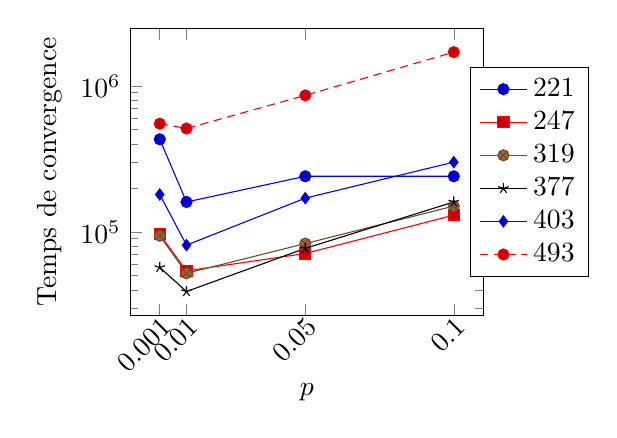
\begin{tikzpicture}
  \begin{axis}[%
      width=0.5\textwidth,
      ymode=log,
      scaled y ticks=false,
      %scaled x ticks=false,
      xlabel={$p$},
      ylabel={Temps de convergence},
      xtick = {0.001, 0.01, 0.05, 0.1%, 0.2
      },
      xticklabel style={ 
        /pgf/number format/fixed,
        /pgf/number format/precision=5,
        inner sep=0pt, anchor=north east, rotate=45 },
      legend entries = {221, 247, 319, 377, 403, 493},
      legend style = {at={(1.3,0.5)}, anchor=east}]
      \addplot coordinates {
        (0.001, 4.3e5) (0.01, 1.6e5) (0.05, 2.4e5) (0.1, 2.4e5) %(0.2, 4.6e5)
      }; 
      \addplot coordinates {
        (0.001, 9.6e4) (0.01, 5.4e4) (0.05, 7.1e4) (0.1, 1.3e5) %(0.2, 1.9e5)
      }; 
      \addplot coordinates {
        (0.001, 9.4e4) (0.01, 5.2e4) (0.05, 8.3e4) (0.1, 1.5e5) %(0.2, 3.0e5)
      }; 
      \addplot coordinates {
        (0.001, 5.7e4) (0.01, 3.9e4) (0.05, 7.7e4) (0.1, 1.6e5) %(0.2, 3.4e5)
      }; 
      \addplot coordinates {
        (0.001, 1.8e5) (0.01, 8.1e4) (0.05, 1.7e5) (0.1, 3.0e5) %(0.2, 8.0e5)
      }; 
      \addplot coordinates {
        (0.001, 5.5e5) (0.01, 5.1e5) (0.05, 8.6e5) (0.1, 1.7e6) %(0.2, 3.6e6)
      }; 

    %\addlegendentry{Temps de convergence}
        
  \end{axis}
  \end{tikzpicture}
  \caption{Temps de convergence moyen en fonction de~$N$ et~$p$ (échelle logarithmique).}
  \label{fig:p_ag}
\end{figure}  

\section{Quelques améliorations}

\subsection{Fixer la taille des diviseurs recherchés}

On  peut donc  envisager l'amélioration  suivante  : plutôt  que d'utiliser  une
grande matrice, on suppose connue la  taille des diviseurs. Si~$n$ est la taille
du nombre à  factoriser, il y a  au plus $4n-2$ tailles de  matrices possibles à
essayer car la somme des  tailles des diviseurs vaut nécessairement~$n$ ou $n+1$
et  on ignore  les  matrices dont  une  dimension vaut~$1$  car  on cherche  des
diviseurs non-triviaux. On  lance donc en parallèle l'algorithme  sur les $4n-2$
matrices différentes, et  on arrête l'exécution dès qu'une  solution est trouvée
pour l'une  des tailles.  Quitte  à supposer impair  le nombre à  factoriser, on
impose  de  plus  qu'il y  ait  un~$1$  à  chacun  des quatre  coins  (condition
nécessairement vérifiée par  la matrice dont les dimensions  sont exactement les
tailles de deux facteurs du nombre à factoriser).
% (c'est une condition
% nécessaire pour qu'une  matrice dont les dimensions sont  exactement les tailles
% de deux  facteurs soit  solution :  chaque facteur commence  par un~$1$  car les
% zéros  à gauche  ne sont  pas  significatifs, et  finissent par  un~$1$ car  les
% diviseurs d'un nombre impair sont impairs).

Il apparaît  que l'exécution de  l'algorithme est significativement  plus rapide
qu'avec la  grande matrice. Les  nombres dont l'un  des facteurs est  très petit
deviennent très  faciles à traiter, car la  matrice de la bonne  taille est très
petite, et le calcul y aboutit  donc rapidement. Les nombres les plus difficiles
à traiter  deviennent, comme pour  les algorithmes classiques  de factorisation,
les  produits de  deux nombres  premiers de  même taille  : en  effet,  la seule
matrice   pour  laquelle  l'algorithme   peut  aboutir   est  alors   de  taille
maximale. Même dans ce  cas, l'exécution est plus rapide car on  ne perd plus de
temps à cause des~$1$ situés dans une zone inutile de la
matrice. %On gagne ainsi un facteur $100$ sur le temps de factorisation de $329$ ($ =7\times 47$), largement de quoi justifier le lancement simultané d'une quinzaine d'exécutions. % TODO : stats plus détaillées ici ?

On donne en Table~\ref{fig:fixedlengths} les temps moyens mis pour atteindre une
solution  pour  certaines  valeurs  de  $N$  par  l'algorithme  initial  et  par
l'algorithme dans lequel  on suppose connue la taille  des diviseurs, lancé avec
la  combinaison de  tailles la  plus favorable  en moyenne.  On tient  compte de
l'ordre des tailles : en effet,  échanger les dimensions de la matrice revient à
transposer la  matrice solution, mais  ce n'est pas  le cas de  la configuration
initiale. Ainsi, il  peut y avoir une différence  de performance significative :
trouver les diviseurs  de $901$ ($=17 \times 53$) est en  moyenne cinq fois plus
rapide sur une  matrice de taille $6\times  5$ que sur une matrice  de taille $5
\times  6$.  On  constate que  la  différence de  performance avec  l'algorithme
initial semble s'accentuer quand $N$ croît : cette amélioration semble permettre
à l'algorithme de passer beaucoup mieux à l'échelle.

\subsection{N'utiliser que des informations locales}

Dans l'algorithme ci-dessus, on utilise des informations globales sur le système lorsqu'on décide si on applique une transformation : en effet, on décide si une case est sûre ou dangereuse en comptant les~$1$ sur la ligne et la diagonale concernées. On peut en fait ajuster l'algorithme pour se restreindre à utiliser uniquement des informations locales, en mettant en place un système de signaux analogue à celui utilisé pour le problème des~$n$ reines. 

On procède de la façon suivante : les cellules de la matrice, en plus de contenir un~$0$ ou un~$1$, peuvent contenir des signaux en provenance des quatre directions~$N$,~$S$,~$E$ et~$W$. On souhaite qu'un signal en provenance d'une certaine direction soit présent sur une cellule si et seulement s'il existe un coefficient égal à~$1$ dans cette direction. Ainsi, une case est dite \emph{sûre} si elle ne contient pas de signal en provenance du nord ni du sud, ou bien si elle ne contient pas de signal en provenance de l'ouest ni de l'est. Dans le cas contraire, elle est dite \emph{dangereuse}. On a ainsi traduit l'ancienne définition d'une cellule sûre (pas de~$1$ sur la même colonne, ou bien pas de~$1$ sur la même ligne) en terme de signaux.

À chaque pas de temps, on choisit une cellule~$c$ à mettre à jour et on commence par mettre à jour ses signaux comme pour le problème des~$n$ reines : pour chaque direction~$d$, si $c'$ est la cellule voisine de~$c$ dans la direction~$d$, le signal en~$c$ en provenance de la direction~$d$ devient présent si $c'$ contient un~$1$, et prend le même état (présent ou absent) que celui de $c'$ en direction de~$d$ sinon.
Après avoir mis les signaux de~$c$ à jour, on applique l'algorithme précédent pour décider si on applique une transformation de $\Gamma$, en utilisant la nouvelle définition de case sûre/dangereuse. 

Comme on pouvait s'y attendre, on constate une légère déterioration des performances lorsqu'on se restreint ainsi à des informations locales : chaque pas de calcul est plus long à réaliser (on doit à la fois appliquer des transformations et mettre à jour des signaux), mais on en fait généralement un peu moins. Dans l'ensemble, le temps de calcul est typiquement doublé. Cette déterioration est néanmoins assez raisonnable, ce qui est prometteur dans le sens où se restreindre à des informations locales peut permettre de paralléliser le système en effectuant plusieurs mises à jour simultanées, sans conflits à condition que les zones affectées par les différentes mises à jour soient disjointes. Ceci était moins efficace avec l'algorithme initial du fait de la nécessité de garder une trace du nombre total de~$1$ sur chaque ligne et diagonale, ce qui impose de centraliser les mises à jour sous peine d'en effectuer certaines avec des informations erronées.

%TODO : comparatif entre fact_fixed_lengths et fact_sigs

\subsection{Permettre des échanges à plus longue distance}

Les transformations  préservant l'invariant de somme introduites  plus haut sont
très  localisées :  on peut  envisager de  remplacer les  règles  \textbf{R1} et
\textbf{R2}  par  une règle  plus  générale,  qui  consiste à  intervertir  deux
cellules situées sur  la même diagonale descendante. De  même, on peut remplacer
les  règles \textbf{R3} et  \textbf{R5} par  une règle  qui consiste  à échanger
un~$1$ d'une diagonale  contre deux sur la diagonale à sa  droite, et les règles
\textbf{R4} et  \textbf{R6} par une règle  qui consiste à  échanger un~$0$ d'une
diagonale  contre deux  sur la  diagonale à  sa droite.  Les  transformations du
système sont ainsi  plus équitables au sens où on  peut maintenant atteindre, en
appliquant  une  seule  règle,  des  positions  qu'on  ne  pouvait  précédemment
atteindre que par une séquence précise de transformations locales.

L'effet de ce  changement sur les performances est mitigé :  dans la plupart des
cas, on constate une amélioration de  l'ordre de $40\%$, mais dans certains cas,
le temps de calcul est au contraire  beaucoup plus grand (ainsi, il est dix fois
plus  long  pour $N=901$).  Par  ailleurs, il  devient  bien  plus difficile  de
paralléliser  les calculs comme  on l'a  envisagé dans  la section  précédente.

\begin{table}[htb]
  \centering
  \begin{tabular}{r|c|c|c|c}
    & algo    & taille des       & et informations  & et déplacements \\
    $ N$ & initial & diviseurs connue & purement locales & globaux\\
    \hline
    \rule{0pt}{3ex}   221     & 1\e{6}  & 8\e{4}       &  6\e{4} & 4\e{4} \\
    403                       & 8\e{4}  & 1\e{4}       & 8\e{3}&  6\e{3}\\ 
    493                       & 5\e{5}  & 1\e{5}       &1\e{5}&  1\e{5}\\
   635                       & $>10^9$ & 3\e{5}       &4\e{5}&  2\e{5}\\
   893                       & 3\e{6}  & 2\e{5}      & 3\e{5}&  2\e{5}\\
    899                       & 1\e{6}  & 8\e{3}      & 9\e{3}&  5\e{3}\\
    901                       & 2\e{7}  & 3\e{6}      & 3\e{6}&  3\e{7}\\
    923                       & $>10^9$ & 3\e{5}&2\e{5}&1\e{5}
  \end{tabular}
  \caption{Temps moyen mis pour atteindre une solution (en nombre d'étapes).}
  \label{fig:fixedlengths}
\end{table}
%\ANNOT{Modifier la dernière phrase car au contraire, c'est l'extension des voisinages, plus éloignée des ACs, qui perd de son intérêt}

%distance à la situation initiale ? 

%TODO : comparatif entre fact_fixed_lengths et fact_global

\section*{Bilan}

%assez peu de puissance de calcul : pas pu tester sur de plus grands nombres... améliorations passent-elles à l'échelle ?

On est parvenu à une formulation cellulaire du problème de la factorisation à l'aide de la multiplication binaire. Étudier expérimentalement le comportement du système a également permis d'identifier des améliorations intéressantes. Enfin, on a pu démontrer l'atteignabilité des solutions à partir d'une position de départ quelconque. En revanche, on n'a pas obtenu de convergence à proprement parler, mais seulement un système qui passe par des solutions. Pour des raisons de puissance de calcul, il a de plus été impossible de faire des tests statistiquement significatifs sur de plus grands nombres : il est difficile d'estimer la complexité de l'algorithme ou même de savoir à quel point il passe à l'échelle. Comme pour le problème des $n$ reines, l'utilisation du hasard permet d'éliminer plusieurs types de blocages tout en conservant des règles d'évolution relativement simples.

% \ANNOT{Faire ressortir les points suivants : 
%   \begin{itemize}
%   \item Formulation cellulaire du problème
%   \item démonstration de l'atteignabilité de la solution
%   \item étude expérimentale du comportement 
%   \end{itemize}
% }


%%% Local Variables:
%%% mode: latex
%%% fill-column: 80
%%% ispell-dictionary: "francais"
%%% mode: flyspell
%%% TeX-master: "rapportStage"
%%% End:
